% нужно перенести отсюда, картинки как обычно в Google draw, ссылки должны все быть https://docs.google.com/document/d/1FsWbe0d41WPVwD9ZtUDNzMLpLnfcXMClDdrN5QOls10/edit?usp=sharing
    
    

    Ключевой задачей биологии 21 века является понимание функционирования хроматина в эукариотических клетках на молекулярном уровне (см. Рисунок \ref{fig:p6_1_f1}.). Именно в хроматине происходят ключевые процессы интерпретации генетической программы клеток, определяющие их развитие и реакцию на изменение внешних условий. Комплексное решение этой задачи, понимание взаимодействия различных генетических и эпигенетических элементов в геноме (энхансеров, промотеров, инсуляторов, локусов, несущих эпигенетические модификации и т.д.) откроет дорогу к пониманию и управлению сложными регуляторными генетическими сетями, на основе которых функционируют клетки человека, животных, растений. Это в свою очередь позволит усовершенствовать методы диагностики и лечения многих заболеваний, осуществлять рациональный подход к генетическому редактированию и проектированию организмов важных с биотехнологической точки зрения.
    
    В частности известно, что многие болезни человека связаны с теми или иными нарушениями работы хроматина. Изменения в энхансер-зависимой экспрессии генов могут привести к развитию многих видов рака, а также сердечных и аутоиммунных заболеваний у людей \cite{nizovtseva_towards_2017}. Нарушение структуры хроматина и его гетерогенность, наблюдаемая при онкологических заболеваниях, позволяет раковым клеткам вырабатывать резистентность к химиотерапии, а воздействия на структуру хроматина активно рассматриваются как один из способов терапии онкозаболеваний \cite{almassalha_macrogenomic_2017}. Также например, петлеобразование в хроматине рассматривается как  лекарственная мишень для лечения бета-талласемий и серповидноклеточной анемии  \cite{krivega_chromatin_2016}.
    
\begin{figure} [H]
    \centering
    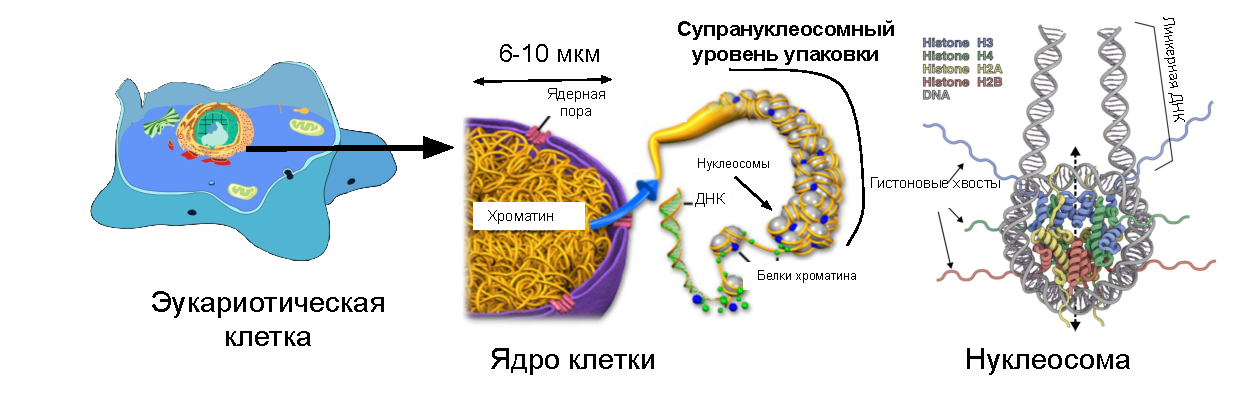
\includegraphics[width=\textwidth]{images/p6/p6_1_vved/p6_1_f1.pdf}
    \caption[От клеток к нуклеосомам.]{От клеток к нуклеосомам. Хроматин находится в ядре эукариотических клеток и включает в себя ДНК, белки и РНК. Элементарная единица упаковки ДНК - нуклеосома, комплекс из 8 гистонов (H3, H4, H2A, H2B) и около 200 пар оснований ДНК. Супрануклеосомальный уровень - уровень укладки нуклеом (от единиц до тысяч нуклеосом, от 200 до 200 000 пар оснований ДНК).}
    \label{fig:p6_1_f1}
\end{figure}
    
\begin{figure} [H]
    \centering
    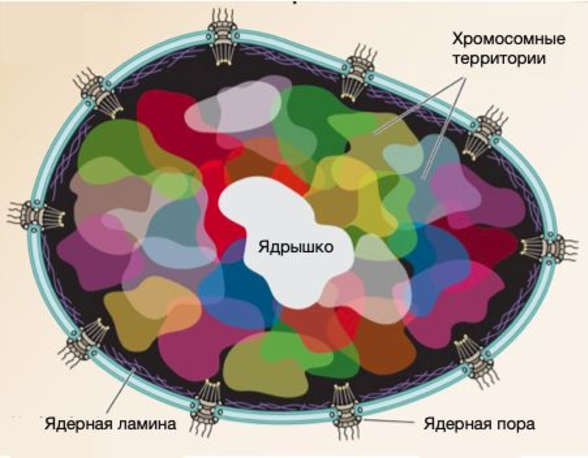
\includegraphics[width=\textwidth]{images/p6/p6_1_vved/p6_1_f2.1.pdf}
    \caption[Хромосомные территории.]{Хромосомные территории. Деконденсированные хромосомы визуализируются (флуоресцентной микроскопией) как хромосомные территории, которые таким образом являются высшим уровнем организации генома. Адаптировано из \cite{fraser_overview_2015}.}
    \label{fig:p6_1_f2.1}
\end{figure}
    
\begin{figure} [H]
    \centering
    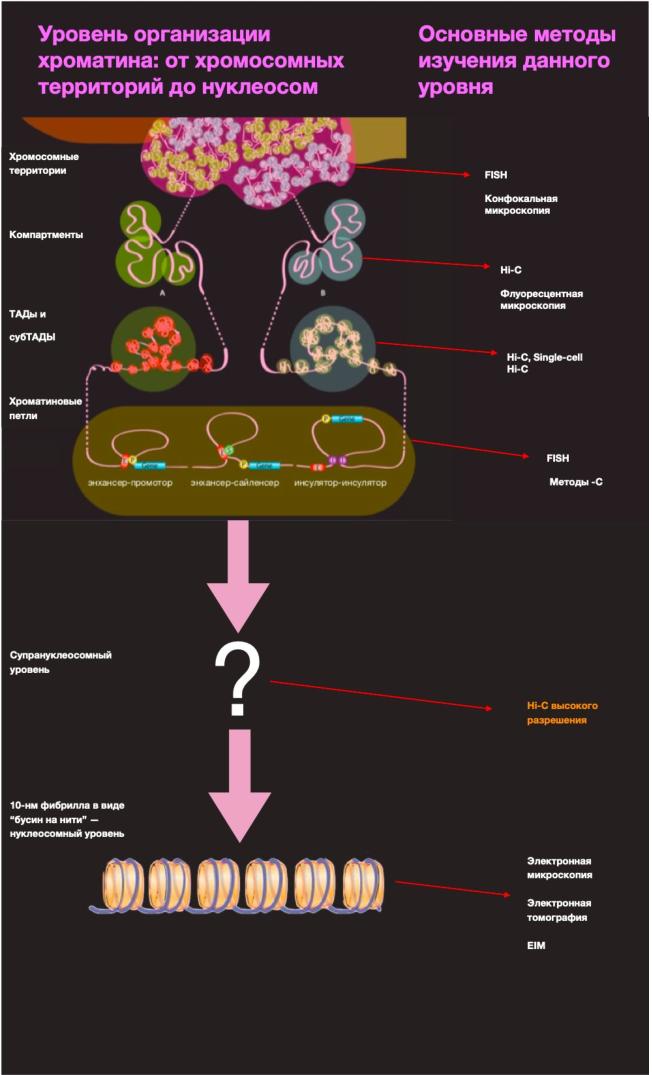
\includegraphics[width=0.5\textwidth]{images/p6/p6_1_vved/p6_1_f2.2.pdf}
    \caption[Структура хроматина и проблема ее понимания на супрануклеосомном уровне.]{Структура хроматина и проблема ее понимания на супрануклеосомном уровне. Представлены следующие за хромосомными территориями уровни организации хроматина и основные методы их обнаружения. Множественные эксперименты с использованием Hi-C говорят о существовании иерархически организованных ТАДов (Топологически ассоциированных доменов) - участков генома, локусы внутри которых чаще физически контактируют друг с другом, чем с локусами извне. Однако о физической природе ТАДов ведутся споры. Их существование пытаются связать с хорошо изученной способностью хроматина к образованию петель и наличием петель, с помощью которых регуляторные элементы генома (сайленсеры, энхансеры) взаимодействуют с регулируемыми ими промотрами генов. Также организацию хроматина на этом уровне пытаются объяснить с позиции коллоидной химии, представляя ключевым для регуляции функциональности хроматина и формирования гетерохроматина переходы между растворимым состоянием и гелеобразным состоянием (через фазу ``жидкой капли'') - модель ``разделения фаз'' \cite{larson_role_2018}.}
    \label{fig:p6_1_f2.2}
\end{figure}
    
    У человека длина всей  ДНК, содержащейся в одной клетке,  равна примерно 2 метрам (0,33 нм длина одного основания, всего около 3.1 млрд. пар оснований). При этом диаметр ядра равен примерно 6 микрометрам. То есть в ядре  ДНК сложена в 3 000 000 раз. При этом она остается функциональной -  гены способны к экспрессии. Однако, эта функциональность избирательна: в разных типах клеток для транскрипции доступны разные гены, их активность определяет уникальность клеточного типа.  Экспрессия контролируется разными способами, но одним  из наиболее важных является специфическая компактизация ДНК в хроматине. Уже с 1907 года известно \cite{gutherz_s._zur_nodate}, что хроматин бывает активным (эухроматин) и неактивным (гетерохроматин), причем последний включает в себя некоторые участки ДНК во всех клетках (конститутивный гетерохроматин), а некоторые - в зависимости от типа и состояния клетки (факультативный гетерохроматин). Эти типы, называемые также активным и неактивным компартментами хроматина, являются уровнем компактизации, следующим за наивысшим - хромосомным (в интерфазе представленном в виде хромосомных территорий, что было открыто с помощью конфокальной микроскопии и FISH -  метода визуализации индивидуальных хромосом на основе флуоресцентной гибридизации и так же хорошо обнаруживающимся с помощью обычной оптической микроскопии. В 1974 году был открыт \cite{kornberg_chromatin_1974-1} низший уровень организации хроматина - нуклеосомный: на нем ДНК наматывается на гистоновые белки, образуя структуру в виде ``бусин на нити'' — 10-нанометровую фибриллу. Этот уровень компактизации ДНК изучен хорошо, в 1997 году методами рентгеновской кристаллографии была определена структура нуклеосомы в атомарном разрешении \cite{luger_crystal_1997}, сейчас накоплено значительное количество данных о биофизике и биохимии нуклеосом и об их цепочках, которые иногда называют 10-нанометровыми фибриллами \cite{hansen_10-nm_2018}. При этом консенсуса об остальных уровнях организации хроматина в научном сообществе нет \cite{maeshima_chromatin_2014,fraser_overview_2015}. Точное представление об уровне, следующем за уровнем компартментов, отсутствует. Как 10-нанометровая фибрилла компактизуется, чтобы образовать хромосому, неизвестно. Долгое время считалось, что она образует 30-нанометровую фибриллу, которая имеет вид соленоида (одностартовая спираль) или зигзага (двустартовая спираль) в зависимости от длины линкерных участков ДНК \cite{perisic_modeling_2010}. Были получены некоторые экспериментальные данные, указывающие на существование данной структуры \cite{tremethick_higher-order_2007,rydberg_chromatin_1998}. Однако на сегодняшний день многие исследователи считают ее артефактной, не существующей \textit{in vivo}. Методы электронной томографии подтверждают существование 10-нанометровой фибриллы, но не 30-нанометровой \cite{razin_chromatin_2014,joti_chromosomes_2012}. Таким образом, организация хроматина на супрануклеосомном уровне остается неясной, поэтому ее изучение является одним из главных вызовов современной молекулярной биологии. 
    
\begin{figure} [H]
    \centering
    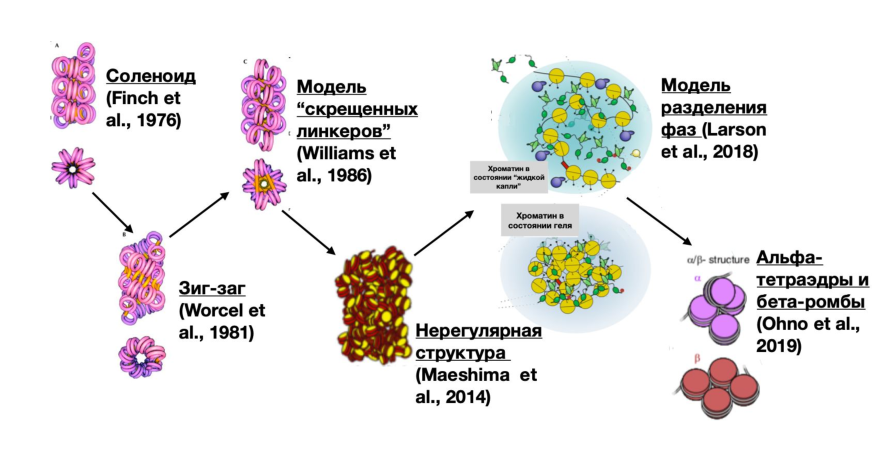
\includegraphics[width=\textwidth]{images/p6/p6_1_vved/p6_1_f3.pdf}
    \caption[О проблеме понимания организации и функционирования хроматина на супрануклеосомном уровне]{О проблеме понимания организации и функционирования хроматина на супрануклеосомном уровне. История представлений об организации супрануклеосомного уровня в хроматине. Использованы иллюстрации из: \cite{wu_variable_2007}; \cite{maeshima_chromatin_2014}; \cite{larson_role_2018}; \cite{ohno_sub-nucleosomal_2019}.}
    \label{fig:p6_1_f3}
\end{figure}
    
    Изучение трехмерной структуры генома имеет очень важное значение для исследования скоординированной работы генов и ее нарушений - например, при онкологических и наследственных заболеваниях, потому что в геноме эукариот существуют регуляторные элементы - последовательности, стимулирующие  - тогда они называются энхансерами - или ослабляющие - их название сайленсеры - экспрессию определенных генов, посредством физического контакта с их промоторами \cite{cavalli_functional_2013,nizovtseva_towards_2017}. Важно, что между регуляторным элементом и регулируемым им геном может быть большое (более мегабазы) геномное расстояние (расстояние в первичной, линейной структуре ДНК). Физический контакт происходит путем образования петли из ДНК \cite{rao_3d_2014}. Для определения наличия физического контакта между последовательностями ДНК в трехмерной структуре генома были разработаны методы семейства -С:3С,4С,5С,Hi-C \cite{fraser_overview_2015}. Эти методы основаны на химическом ``сшивании'' контактирующих в хроматине участков, фрагментации ДНК с образованием ``сшитых'' пар, лигирование фрагментов в этих парах с образованием гибридных молекул ДНК, детекция гибридных молекул (обнаружение молекулы, состоящей из последовательности А и последовательности В, говорит о физическом контакте этих последовательностей в ДНК). Метод 3С позволял оценить взаимодействие только двух участков генома друг с другом, поэтому его называли ``один против одного''. Аналогично: 4С — ``один со многими'', 5С — ``многие со многими''. Наиболее совершенным является метод Hi-C, модифицированный стадией биотинилирования гибридных молекул для обогащения ими раствора путем стрептавидинового осаждения и использованием высокоэффективного секвенирования спаренных концов \cite{lieberman-aiden_comprehensive_2009}. Hi-C - это ``все против всех''. Этот метод позволяет составить матрицу частот взаимодействий между всеми участками генома заданной длины. Метод Hi-C позволил обнаружить следующий за компартментами уровень компактизации хроматина - Топологически ассоциированные домены (ТАДы) - регионы ДНК, в пределах которых взаимодействие участков друг с другом происходит чаще, чем с участками из других регионов\cite{dixon_topological_2012}.
    
    Хотя ТАДы проявляются как определенный паттерн на матрице взаимодействий, их физическая природы неясна \cite{pal_hi-c_2019}. Существуют две основные концепции относительно нее. Первая - DNA loop extrusion (``выпетливания ДНК'') предполагает возникновение на участке ДНК, ограниченном сайтами связывания белка CTCF, петли, расширяющейся со временем до этих сайтов \cite{sanborn_chromatin_2015}. В разных клетках петля в пределах сайтов связывания CTCF находится на разных стадиях расширения - соответственно в разных клетках рядом оказываются разные участки ДНК, что на матрице Hi-C отображается как ТАД. Слабость этой гипотезы в том, что она считает ТАДы популяционным феноменом, в то время как интрахромосомные ТАДы (в отличие от интерхромосомных) и хроматиновые глобулы, считающиеся соответствующими ТАДам, обнаруживаются и в отдельных клетках \cite{nagano_single-cell_2013}. Другая гипотеза утверждает, что ТАДы - это особые хроматиновые домены, возникающие в клетках из-за физического взаимодействия между нуклеосомами в неактивном хроматине \cite{ulianov_active_2016}. Эта гипотеза тоже имеет недостаток - она не объясняет расположения сайтов связывания CTCF на границах ТАДов. Таким образом очевидно, что необходимо продолжать исследования структуры хроматина и на уровне ТАДов. Так как ТАДы отчасти ``фрактальны'' -  содержат внутри себя вложенные друг в друга ТАДы меньших размеров - изучение хроматина даже на супрануклеосомном уровне может помочь понять структуру всей иерархии ТАДов \cite{phillips-cremins_architectural_2013,norton_detecting_2018}. 
    
    Для исследований регуляторной функции хроматина необходимо понимать его супрануклеосомальную организацию. Так, обеспечение коммуникации между энхансером и промотером, которые могут располагаться на расстояниях до нескольких сотен килобаз, обеспечивается за счет образования петель. Энхансеры - элементы, которые обеспечивают транскрипционную активацию подавляющего большинства генов человека и в значительной степени определяют состояние хроматина вблизи промоторных областей. Эпигенетическими метками активных энхансеров явяются, в частности, H3K27ac, H3K4me1, H3K27me3, и гистоновые варианты H3.3 и H2A.Z. К меткам промотеров относятся: H3K4me3 и H3K27ac \cite{nizovtseva_towards_2017}. 
    
    Исследования энхансеров затрудняются их различиями в последовательности ДНК. Большинство промотеров ассоциировано с 1 энхансером, в то время как 25\% промотеров - с двумя или больше в разные моменты времени. Известно более миллиона энхансеров, а одновременно активны порядка тысячи энхансеров. 
    
    Изменения в энхансер-зависимой экспрессии генов могут привести к развитию многих видов рака, а также сердечных и аутоиммунных заболеваний у людей. К изменению активности энхансеров в онкологических заболеваниях  приводит изменение копийности энхансеров, структурные перестройки генома, изменяющие таргетный ген энхансера и точечные мутации или индели, которые влияют на связывание с транскрипциоными факторами и образовывают новые энхансеры или наоборот, разрушают инсуляторы \cite{sur_role_2016}. 
    
    Актуальной проблемой в области лечения онкологии, в части в химиотерапии, является развитие резистентности к лекарственным агентам. Так, в работе \cite{almassalha_macrogenomic_2017} было показано, что использование агентов, влияющих на внутриядерные изменения плотности упаковки хроматина, приводит к уменьшению транскрипционной гетерогенности и, соответственно, к предотвращению возникновения химиорезистентности. 
    
 \subsection{О прогрессе методов структурной биологии в изучении супрануклеосомной организации} 

    Кристаллическая структура коровой частицы нуклеосомы (гистоны H3, H4, H2A, H2B и 145-147 пар оснований ДНК) с атомистическим разрешением была получена в 1997 году \cite{luger_crystal_1997} (Рисунок \ref{fig:p6_1_f4}). Позднее стало очевидно, что данная структура является лишь некоторым компактным вариантом, который удовлетворяет условиями кристаллической упаковки, а сама нуклеосома достаточно динамична. Несмотря на биохимические данные о динамичности нуклеосом, получения различных вариантов ее структуры в динамике стало возможным лишь недавно благодаря успехам криоэлектронной микроскопии \cite{bilokapic_structural_2018}. Также благодаря криоэлектронной микроскопии в последние годы получены разнообразные структуры нуклеосом с белками хроматина, в частности структура нуклеосомы при прохождении РНК-полимеразы \cite{ehara_structural_2019}, структуры нуклеосом с различными ремоделлерами (белковыми комплексами перемещающими нуклеосомы или заменяющими гистоны) \cite{farnung_nucleosomechd1_2017,li_mechanism_2019,yan_structures_2019}.
    
    Важной вехой явилось определения структуры хроматосомы - комплекса нуклеосомы с линкерным гистоном H1 \cite{bednar_structure_2017}.
    
    Применение криоЭМ к определению структуры нуклеосомальных фибрилл также проводилось. Были получены структуры нуклеосмных фибрилл с и без гистона H1 \cite{song_cryo-em_2014}. Однако, данные фибриллы, состоящие из 12 нуклеосом, находящихся на равном расстоянии друг от друга, были приготовлены искусственно. Поэтому значение данной структуры для понимания биологических процессов ставится под сомнение.

\begin{figure} [H]
    \centering
    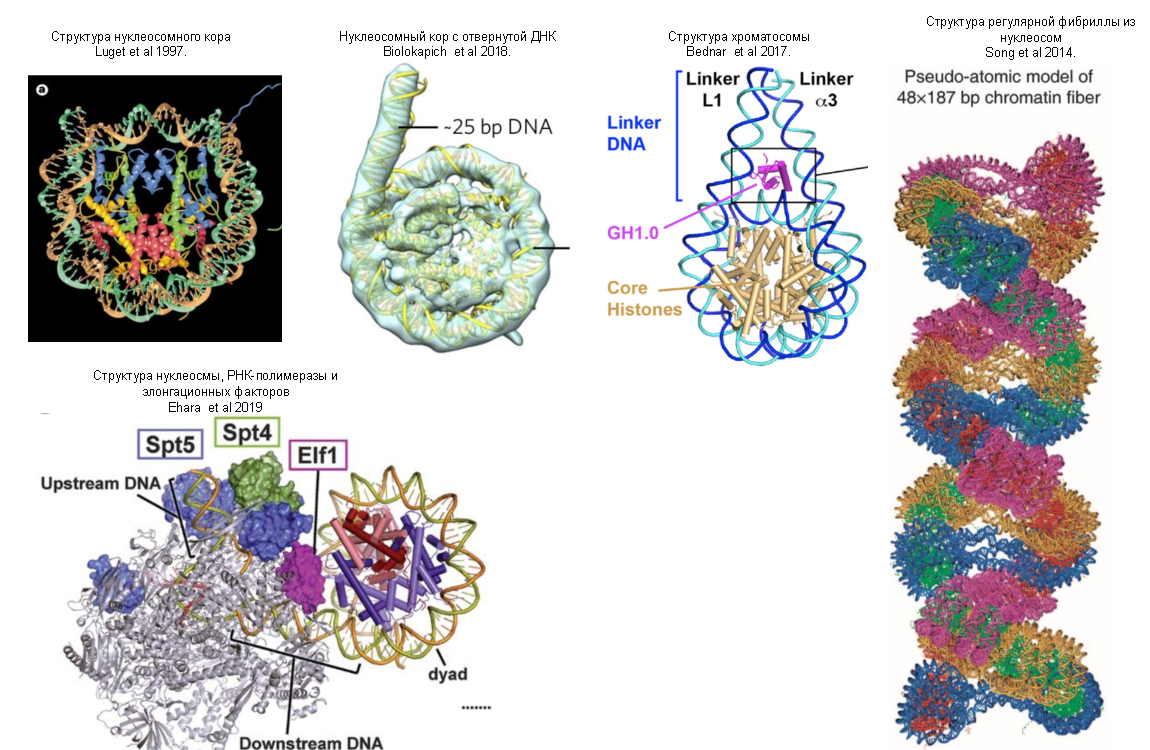
\includegraphics[width=\textwidth]{images/p6/p6_1_vved/p6_1_f4.pdf}
    \caption{Различные структуры нуклеосом, их комплексов и фибрилл из нуклеосом, полученные в последнее время методами структурной биологии.}
    \label{fig:p6_1_f4}
\end{figure}
    
    
    
    
    
    
    
    
    
    
    
    
    
    
    
    
    
    
    
    
    
    
    
    
    
    
    
    
    
    
    
    
    
    
    
    
    
    
    
    
    
    
    
    
    
    
    
    
    
    
    
    
    
    
    
    
    
    
    
    
    
    
    
    
    
    
    
    
    
    